\begin{figure}[tbp]
\centering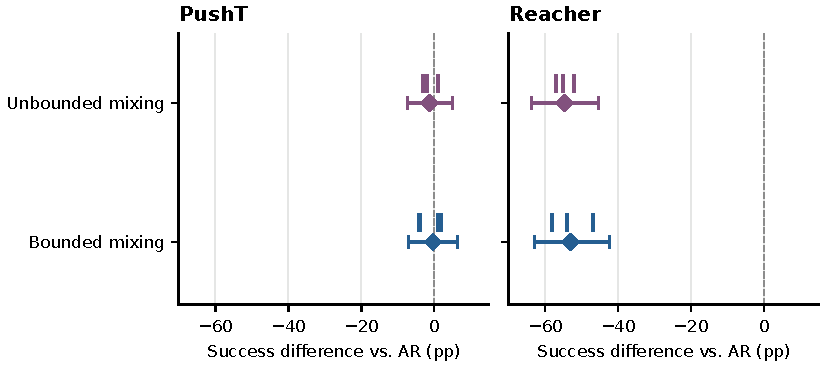
\includegraphics[width=\linewidth]{generated/iclr_review_v1/planning_seed_robustness.pdf}
\caption{Current-model control is not a general benefit of observed-state mixing.
Diamonds show success differences against matched autoregression; whiskers are
the original paired seed--episode 95\% bootstrap intervals. Small vertical marks
show each of the three training-seed differences. All 100 held-out starting
episodes per task are retained. Reacher regressions occur for every seed in both
mixing arms; the PushT intervals include zero. This secondary display does not
change the model selection, primary endpoint or test population.}
\label{fig:planning-seed-robustness}\end{figure}
